\begin{figure*}[!ht]
    \centering
     \subfloat[Loss with different bitwidth]{
        \label{fig:Loss_with_bits}
        \begin{minipage}[t]{0.3\textwidth}
            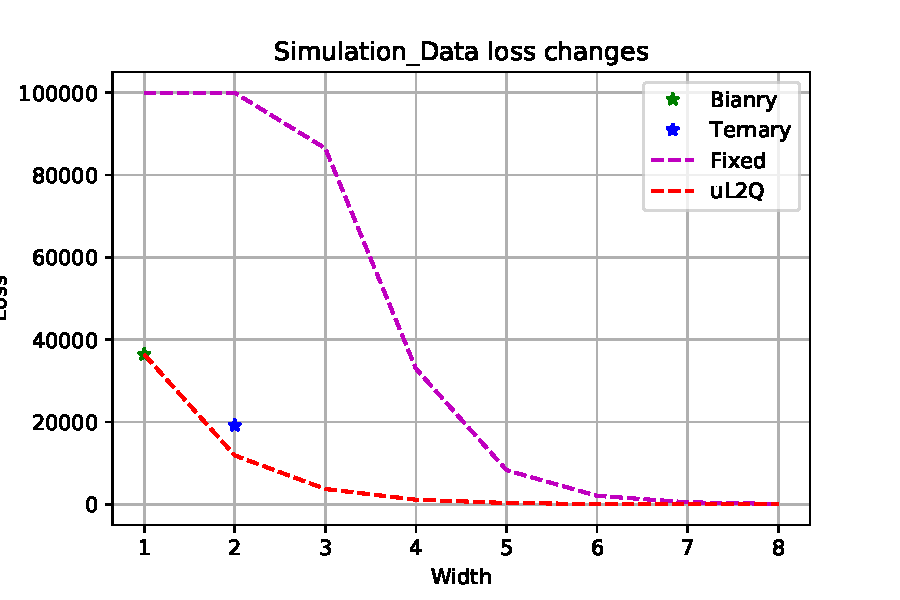
\includegraphics[width=1\textwidth]{Simulation/Bitwidths/LossWithWidth.pdf}
        \end{minipage}
     }
     \subfloat[Loss with different means]{
        \label{loss_with_means}
        \begin{minipage}[t]{0.3\textwidth}
        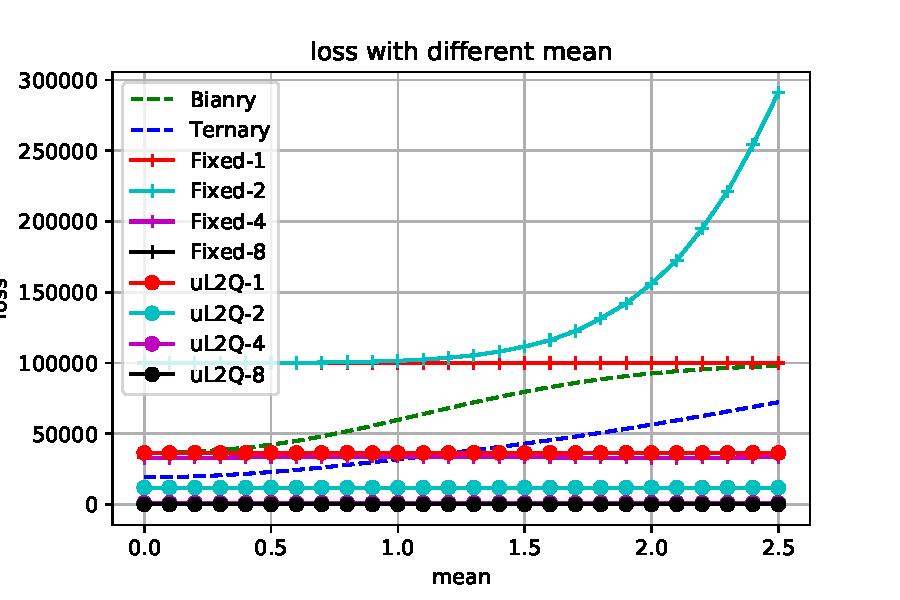
\includegraphics[width=1\textwidth]{Simulation/ShiftScale/loss_with_mean_in_small_range.pdf}
        \end{minipage}
     }
     \subfloat[Loss with different standard deviations]{
        \label{loss_with_sds}
        \begin{minipage}[t]{0.3\textwidth}
        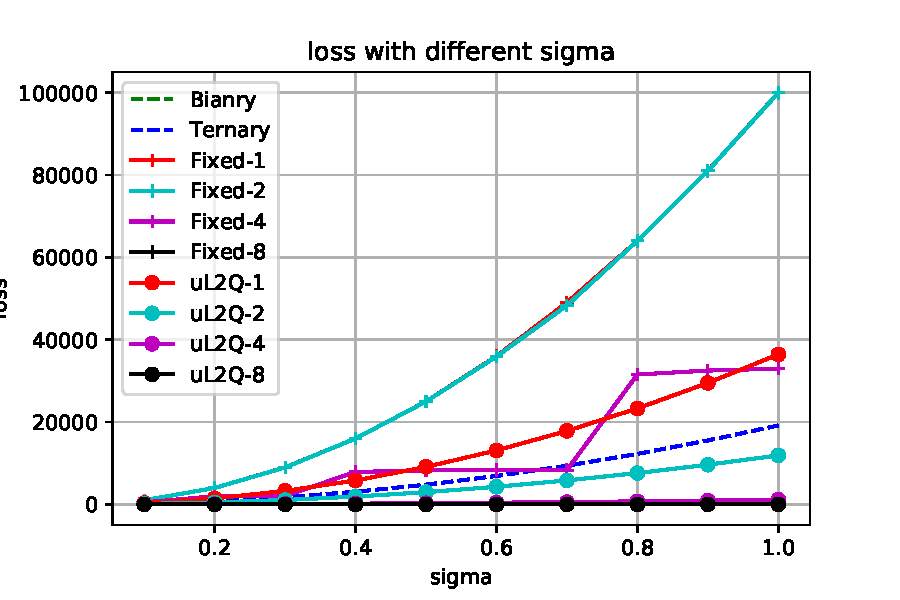
\includegraphics[width=1\textwidth]{Simulation/ShiftScale/loss_with_sigma_in_small_range.pdf}
        \end{minipage}
     }
    \caption{Losses for different means and standard deviations.}
    %distributions. The result of the fixed-point quantization at 8-bit width coincides with the 4-bit and 8-bit width results of our method. Our method is insensitive to mean change and is the most stable for standard deviation changes.}
    \label{fig:loss_with_distribution}
\end{figure*}
\section{Evaluations}\label{sec:exp}
We use both simulated data and DNN model training to evaluate our proposed $\mu$L2Q method.
%The experimental part are divided into three experimental parts: \textbf{simulated distribution analysis}, \textbf{DNN weights analysis} and \textbf{DNN training}. 
\textbf{Simulated data} is used to evaluate the data loss of different quantization algorithms from existing works as well as our proposed solution. 
%Since the generation of analog data is relatively easy, this part of the experiment can comprehensively analyze the comparison results of different quantization algorithms under all different distribution cases.
In the \textbf{DNN model} based evaluations, we first analyze our quantization on some selected model weights trained without our quantization to show the effectiveness of our method. We then illustrate our quantization method as a solution in the current Caffe \citep{jia2014caffe} framework and enabled it for model training and use the final trained accuracy of the models to demonstrate the impact of our $\mu$L2Q method for data quantization. The version of Caffe framework is 1.0.0.

\subsection{$\mu$L2Q on Simulated Data}
\subsubsection{Experimental settings}
We randomly generate $N=100000$ data with normal distribution $\mathcal N(\mu, \sigma^2)$
and consider the impact of 
(1) targeted bit widths, (2) mean value for normal distributions with $\sigma=1.0$ and (3)standard deviations for the normal distribution with $\mu$ set to 0, on the quantized results.
\subsubsection{Loss for different bitwidth}

%TODO: squeeze these two figures into sigle co
%\begin{figure}[!]
    %\centering
    % \subfloat[Data distribution]{
        % \label{fig:dist}
        % \begin{minipage}[t]{0.48\textwidth}
% 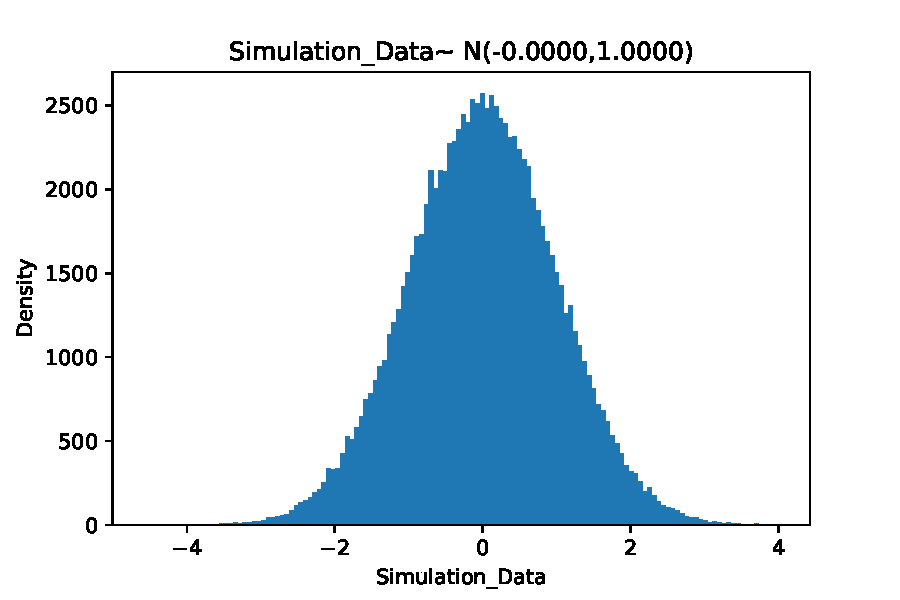
\includegraphics[width=1\textwidth]{Simulation/Bitwidths/Distribution.pdf}
        % \end{minipage}
    % }
    % \subfloat[Loss with different bit widths]{
        % \label{fig:loss}
        % \begin{minipage}[t]{0.48\textwidth}
        %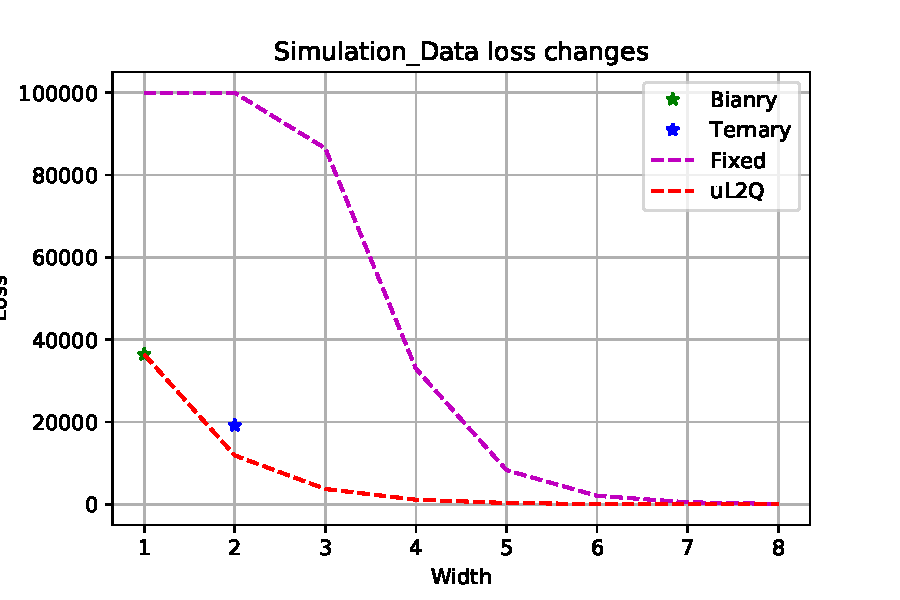
\includegraphics[width=0.48\textwidth]{Simulation/Bitwidths/LossWithWidth.pdf}
        % \end{minipage}
    % }
    %\caption{Loss with different bitwidth.}
    %For the same data distribution, as shown in \figref{fig:dist}, the loss comparison of different quantization algorithms over different bit widths. From \figref{fig:loss}, Our quantization algorithm has the lowest loss in all bit widths.}
    %\label{fig:Loss_with_bits}
%\end{figure}

As shown in~\ref{fig:Loss_with_bits},
our quantification method maintains the lowest data loss over all bit widths. 
For binary quantization, which the quantized data occupied only 1 bit, we maintain the same data loss as~\cite{zhou2016dorefa}. It is worth noting that the loss of our method does not change with the mean value of the original data, 
but binary quantization in~\cite{zhou2016dorefa} could only provide a minimum data loss when the mean value is zero according to our experimental results.

The ternary quantizatio, the quantized data occupies 2 bits, the data loss of $\mu$L2Q at 2 bit is lower than the state-of-the-art results from~\cite{TWNs}. 
Ternary uses 2-bit resource to represent three values \{-1, 0, 1\}. Meanwhile, $\mu$L2Q fully use 2 bits with four values \{-1, 0, 1, 2\}. Therefore, the data loss of $\mu$L2Q is lower.

The loss of $\mu$L2Q is always lower than the fixed point quantization. The reason is that fixed point quantitation does not consider the normal distributed data characteristic. $\mu$L2Q take the data distribution into consideration and provides a more balanced quantization. 

%Fixed-point quantization can be performed on different quantization bit widths, but its high loss at low bit widths and its low utilization of bit width make it difficult to achieve better trade-offs between efficiency and loss.

% \begin{figure*}[!ht]
%     \flushleft
%     \begin{minipage}[t]{1\textwidth}
%             \flushleft
%             \begin{overpic}[width=0.24\textwidth]{Simulation/Bitwidths/BinaryDistribution.pdf}
%                 \put(-10,15){\rotatebox{90}{Binary}}
%                 \put(93,15){\rotatebox{90}{Ternary}}
%                 \put(-10,-50){\rotatebox{90}{Fixed}}
%                 \put(-10,-115){\rotatebox{90}{Our}}
%                 \put(40,70){1bit}
%                 \put(145,70){2bit}
%                 \put(250,70){4bit}
%                 \put(355,70){8bit}
%             \end{overpic}
%             %\includegraphics[width=0.24\textwidth]{fig/SingleFmeasure/bark_f1_single.pdf}
%             %\includegraphics[width=0.24\textwidth]{fig/Bitwidths/binary-results_1bit.pdf}
%             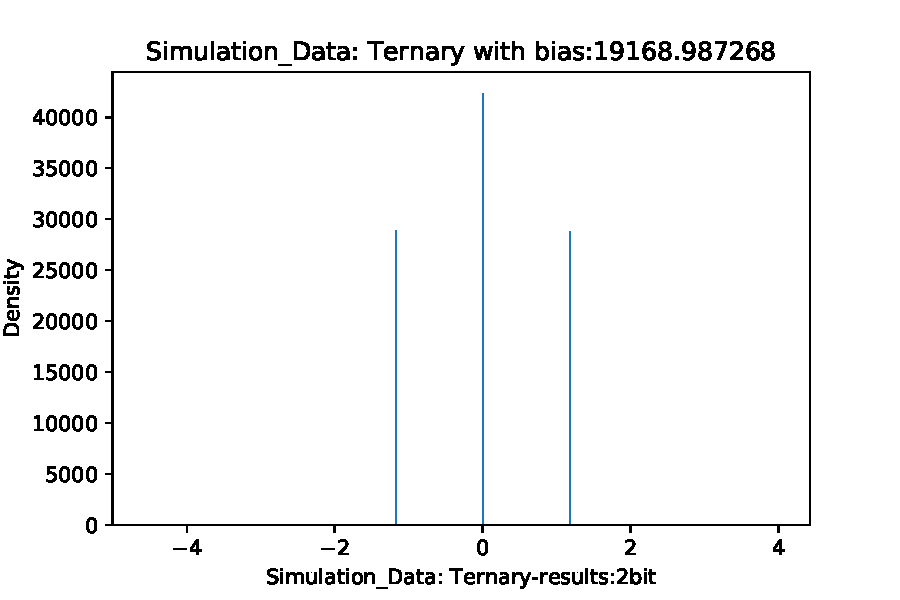
\includegraphics[width=0.24\textwidth]{Simulation/Bitwidths/TernaryDistribution.pdf}\\
%             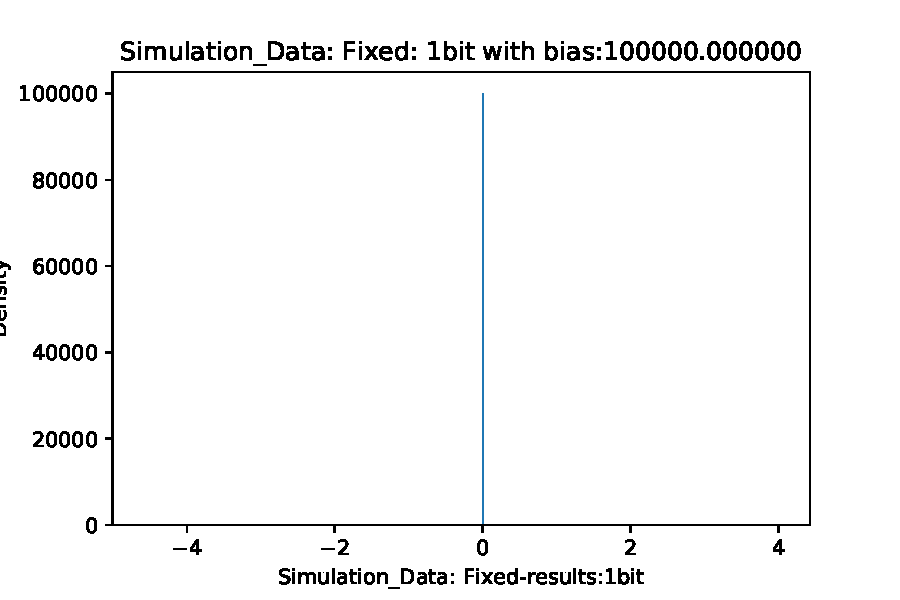
\includegraphics[width=0.24\textwidth]{Simulation/Bitwidths/FixedDistribution_1bit.pdf}
%             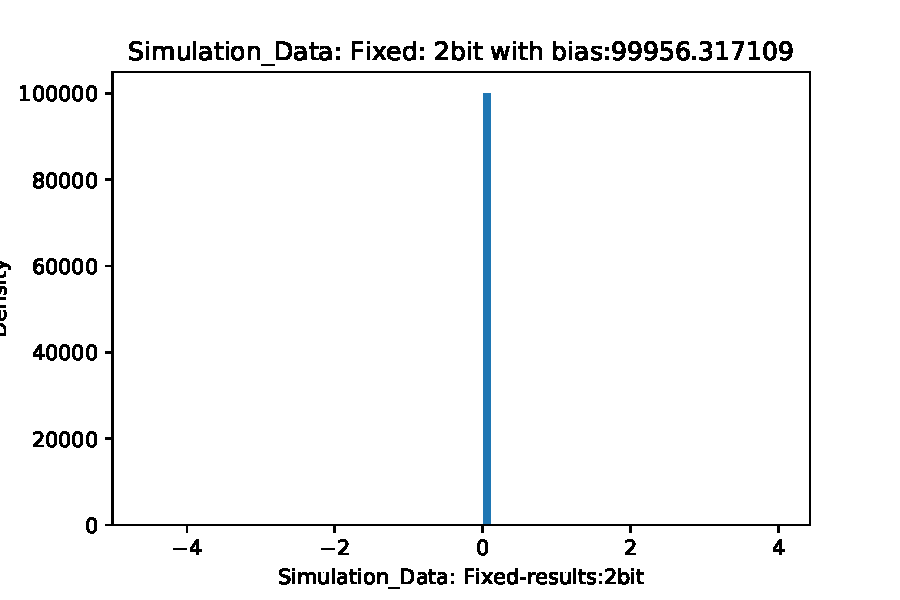
\includegraphics[width=0.24\textwidth]{Simulation/Bitwidths/FixedDistribution_2bit.pdf}
%             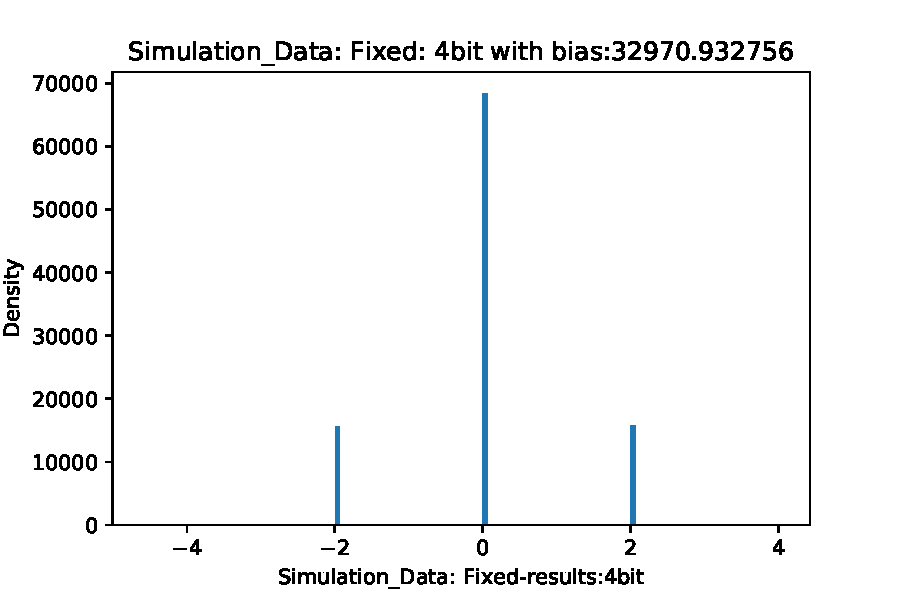
\includegraphics[width=0.24\textwidth]{Simulation/Bitwidths/FixedDistribution_4bit.pdf}
%             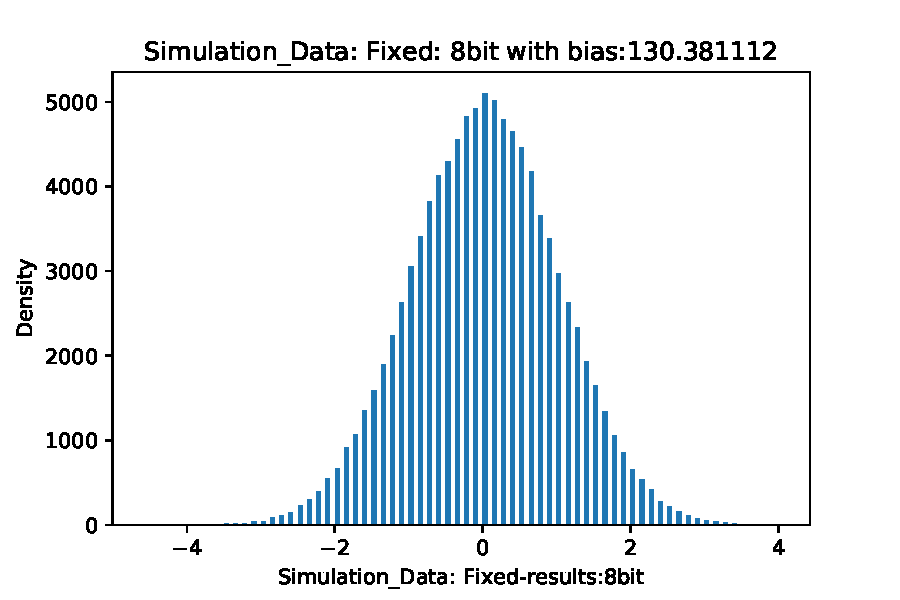
\includegraphics[width=0.24\textwidth]{Simulation/Bitwidths/FixedDistribution_8bit.pdf}\\
%             \includegraphics[width=0.24\textwidth]{Simulation/Bitwidths/$\mu$L2QDistribution_1bit.pdf}
%             \includegraphics[width=0.24\textwidth]{Simulation/Bitwidths/$\mu$L2QDistribution_2bit.pdf}
%             \includegraphics[width=0.24\textwidth]{Simulation/Bitwidths/$\mu$L2QDistribution_4bit.pdf}
%             \includegraphics[width=0.24\textwidth]{Simulation/Bitwidths/$\mu$L2QDistribution_8bit.pdf}
%             %\fbox{\rule[-. 5cm]{0cm}{4cm} \rule[-. 5cm]{4cm}{0cm}}
%     \end{minipage}
%     \caption{Quantized data distribution, original data distribution is shown in \figref{Data_distribution}. Compared with other quantization algorithms, our algorithm makes full use of the expression ability within the set bit width to quantize the original data to the maximum amount of information that can be carried by the set bit width.}
%     \label{fig:quantization_distribution}
% \end{figure*}

\subsubsection{Loss with different means and standard deviations}
%The actual network weights are often not standard normal distributed, and it is necessary to test the performance of the quantization algorithms on different normal distributions.
%Different quantization methods should be stable and robust on different normal distributions. We generate normal distribution data with different mean and standard deviations to test the performance of different quantization methods.
%\textbf{Results: }
As shown in \figref{fig:loss_with_distribution}, Our method is the most stable one among all the evaluated methods with the different means and standard deviations.
The loss of binary and ternary quantization increase as the mean shifts away from the origin, as is shown in~\figref{loss_with_means}.
%The fixed-point quantization does not support 1 bit due to the sign value but we still put the value there to ease comparison of the following values.
%is stable in 1 bit since fixed-point quantization can only be quantized to 0 when the bit width is 1 bit, that is, the sign bit. 
%\textcolor{red}{Remove the 1 bit for fixed, it does not support 1 bit.}
Fixed-point quantization fluctuates greatly at 2bit width, while it is stable at 4-bit and 8-bit since the bit width is sufficient for data representation. 
The data loss of $\mu$L2Q does not change with the mean value. What is more, the data loss of $\mu$L2Q at 1 bit can even achieve the same as fixed-point quantization with 4 bits data representation. 
%When the mean value is greater than 1, our method shows lower loss than any other methods.
Our method is also shows the most stability among all the other quantization methods with different standard deviations by taking advantage of taking the data distribution into consideration, as shown in \figref{loss_with_sds}. 
% As the standard deviation increases, the difference of data is prominent, and the loss of all quantization methods increases. The fixed-point quantified fluctuation is the greatest, and our method coincides with binary quantization at 1 bit width. Our method is the most stable, and the results at 2bit width has better than binary, ternary quantization, and fixed-point quantization's results at 4bit width.

%can achieve the lowest loss is that we fully consider the three factors: 1) Based on the standard normal distribution, we theoretically fully analyze the optimal choice of the quantized locations, which is the essential reason for our algorithm achieving the lowest loss; 2) We normalize all the data to the standard normal distribution and then quantify it, which not only ensures the premise of our theoretical analysis above, but also ensures that our method is insensitive to mean and keep stable for standard deviation change, which guarantees the robustness of our method; 3) We make full use of the bit-width resources, without wasting any representation bits. Our method can make full use of $2^k$ representation values for $k$-bit width resources. For example, as shown in \figref{fig:quantization_distribution}, on 1bit, our method quantizes to 2 values; on 2bit quantizes to 4 values, and the values are 16 and 256 on 4bit and 8bit respectively. In contrast, ternary quantization only uses 3 values of the 4 values, and the fixed-point quantization method has also no relevant guarantee.



\subsection{$\mu$L2Q for DNN training}
%数据集的选择
\subsubsection{Experimental settings}
% \textbf{Selection of datasets.}
Three well-known data sets are chosed for our experiments, which are Mnist \citep{mnist}, Cifar10 \citep{cifar10} and ImageNet \citep{deng2009imagenet}. 
% The size of the images in the three data sets is incremental, Mnist is the smallest, Cifar10 is larger, and ImageNet is the largest. 
% These three data sets are often used to evaluate the effectiveness of the compression method such as in \citep{TWNs,gysel2016hardware,Ternaryconnect}.
%基于数据集的网络模型选择
% \textbf{Selection of DNN models.}
Based on the above datasets, we select some widely used neural network models for our evaluations, including Lenet-5 \citep{lecun1998gradient} for Mnist, Cifarnet \citep{krizhevsky2009learning} and VGG7-64 \citep{simonyan2014vgg}\footnote{Network architecture is $3\times32\times32 (input)-C(3,64)-BN-C(3,64)-BN-MP2-C(3,128)-BN-C(3,128)-BN-MP2-C(3,256)-BN-C(3,256)-BN-F(1024)-BN-F(10)-Softmax$. C(K,O) denotes a convolution with kernel size $K\times K$ and $O$ outputs, MP2 stands for $2\times2$ max pooling, F(O) means the fully-connected layer with $O$ outputs, and BN represents batch normalization. 
} 
for Cifar10 and Resnet-18 \citep{he2016deep} for ImageNet. The effectiveness of our proposed method is evaluated with the illustration of it into Caffe training flow. 
% The final testing accuracy is the comparison metric. 
The network size in terms of parameter number and training settings for different models are shown in \tabref{tab:networktrainingmodel}.
\begin{table}[]
\caption{Model size and training parameter settings.}
\label{tab:networktrainingmodel}
\begin{tabular}{c|c|c|c|c}
\hline
Dataset                   & Mnist  & \multicolumn{2}{c|}{Cifar10} & Imagenet  \\\hline
Model                     & Lenet5 & Cifarnet     & VGG7-64      & Resnet-18 \\\hline
Parameter number(M)             & 0.43 & 0.279      & 5.35       & 11.69   \\\hline
Weight decay              & 0.0004 & 0.0001       & 0.0004       & 0.0001    \\
Batch size                & 100     & 100          & 100          & 64*4      \\
Initial learning rate     & 0.01   & 0.0001       & 0.01         &   0.1        \\
Learning rate decay & 0.1  & 0.1    & 0.2     &         0.1  \\
Learning rate decay epoch & 32,48  & 120,130      & 16,32,36     &     30,40,50      \\
Momentum                  & 0.9    & 0.9          & 0.9          & 0.9    \\\hline  
\end{tabular}
\end{table}

\textbf{Existing quantization methods for comparing.}
Many existing quantization methods including the state-of-the-art ones are chosen for comparison.
These methods can be divided into three categories. 
Firstly, binary quantization methods, including RebNet \citep{ghasemzadeh2018rebnet}, BNN \citep{BitwiseNN}, BPWNs \citep{TWNs}, BWN \citep{rastegari2016xnor}, XNOR-NET \citep{rastegari2016xnor} and BC \citep{Binaryconnect}. 
Secondly, ternary quantization methods are chosen, including TNN \citep{alemdar2017ternary}, TN \citep{TrueNorth1}, TWNs \citep{TWNs}, STC \citep{jin2018sparse} and TC \citep{Ternaryconnect}. 
Finally, some certain bitwidths of fixed-point quantization results from hardware~\cite{gysel2016hardware} are also chosen to compare with the results of our $\mu$L2Q. 
All the comparison targets are concluded in \tabref{tab:comparisionmethods}.
\begin{table}[]
    \centering
    \caption{Comparison targets.}
    \label{tab:comparisionmethods}
    \begin{tabular}{c|c}
        \hline
        Category & Methods \\\hline
        \multirow{2}{*}{Binary} & RebNet \citep{ghasemzadeh2018rebnet}, BNN \citep{BitwiseNN}, BPWNs \citep{TWNs}, \\
                & BWN \citep{rastegari2016xnor}, XNOR-NET \citep{rastegari2016xnor}, BC \citep{Binaryconnect}\\\hline
        Ternary & TNN \citep{alemdar2017ternary}, TN \citep{TrueNorth1}, TWNs \citep{TWNs}, STC \citep{jin2018sparse} and TC \citep{Ternaryconnect} \\\hline
        Fixed-point& hardware \cite{gysel2016hardware}\\\hline
        \textbf{Ours}&$\mu$L2Q\\\hline
    \end{tabular}
\end{table}

\textbf{Training configuration and result settings of $\mu$L2Q.} 
$\mu$L2Q can achieve data quantization at any bit width. 
For simplicity of description, we use $\mu$L2Q-x to denote $\mu$L2Q quantized data at x-bit width.
$\mu$L2Q-x compresses the network's weights, including weights of convolution and fully-connected layer to x-bit width. 
However, considering that the last fully-connected layer has a greater impact on the accuracy of the model, we only quantize the last fully-connected layer to 8/16 bits or maintain it as floating point.

\begin{figure*}[htp]
\centering
\subfloat[Lenet5]{
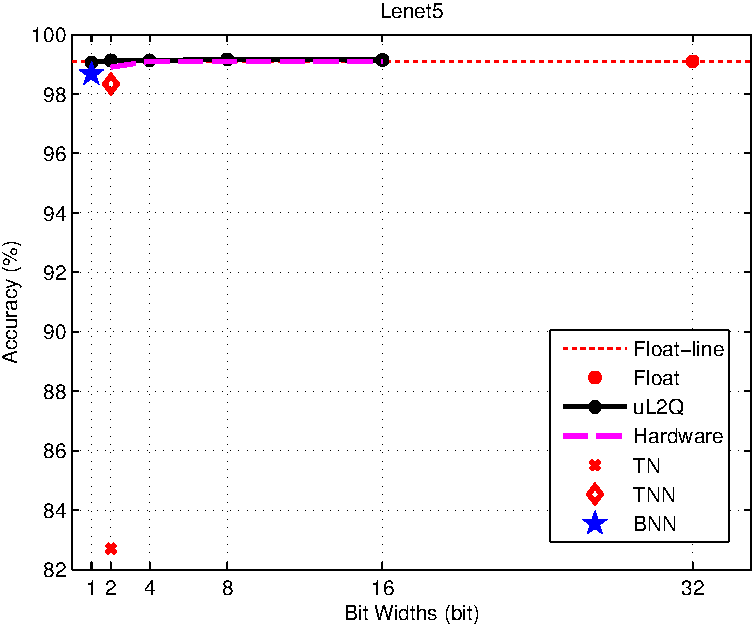
\includegraphics[width=0.31\textwidth]{fig/Lenet5_accuracy_bits.pdf}
\label{fig:lenet5acc}
}
\subfloat[Cifarnet]{
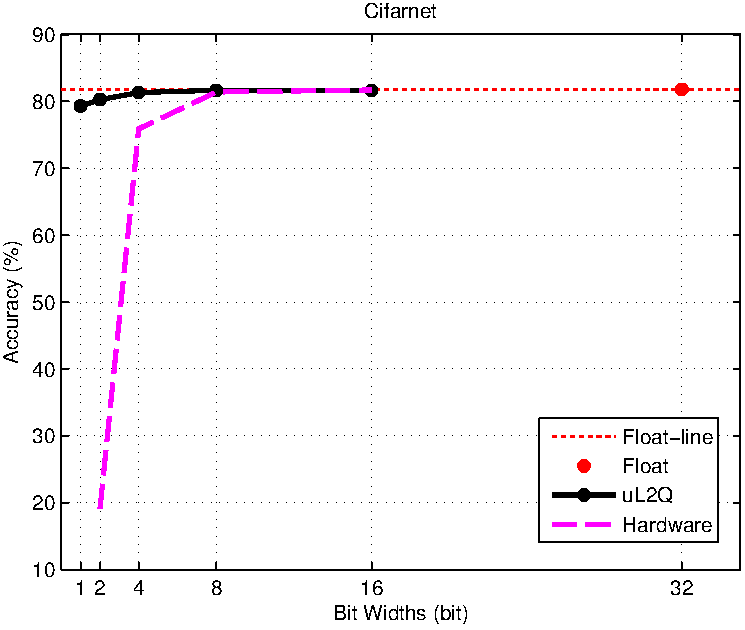
\includegraphics[width=0.31\textwidth]{fig/Cifarnet_accuracy_bits.pdf}
\label{fig:cifarnetacc}
}
\subfloat[VGG7-64]{
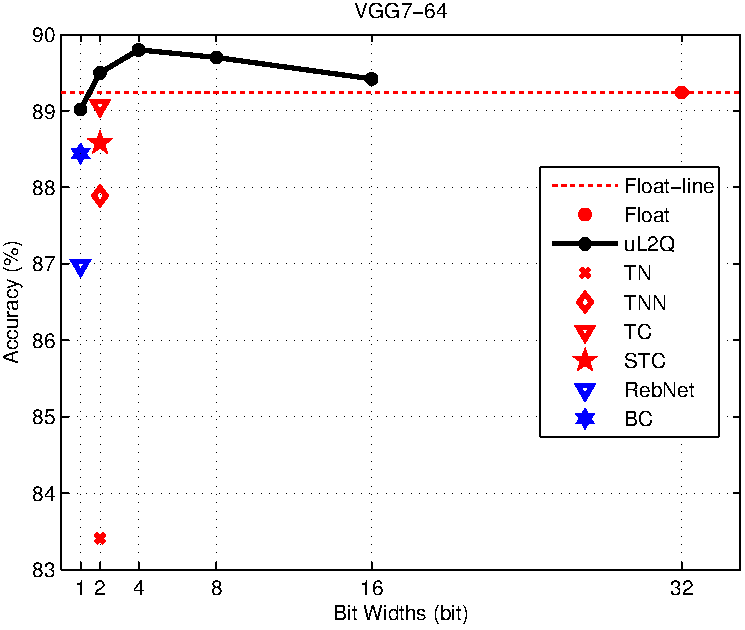
\includegraphics[width=0.31\textwidth]{fig/VGG7-64_accuracy_bits.pdf}
\label{fig:vgg764acc}
}\\
\subfloat[ResNet-18 Top1]{
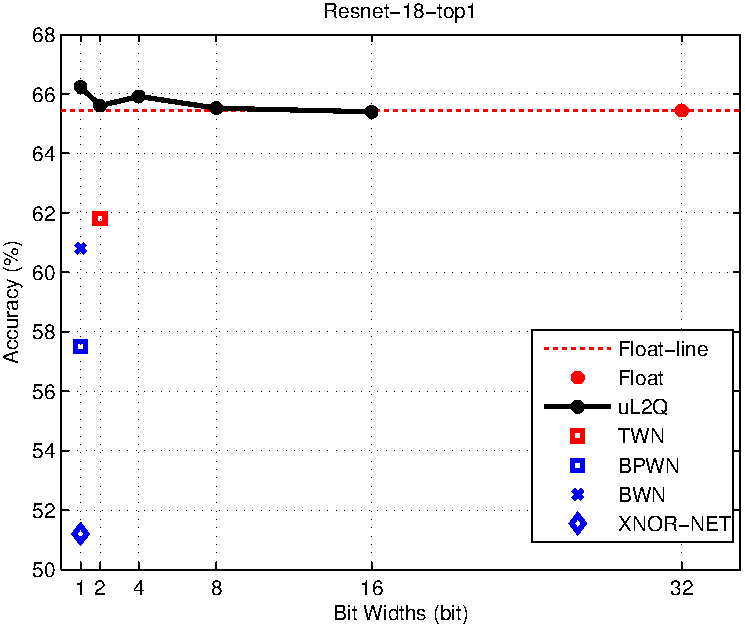
\includegraphics[width=0.31\textwidth]{fig/Resnet-18-top1_accuracy_bits.pdf}
\label{fig:resnet181acc}
}
\subfloat[ResNet-18 Top1]{
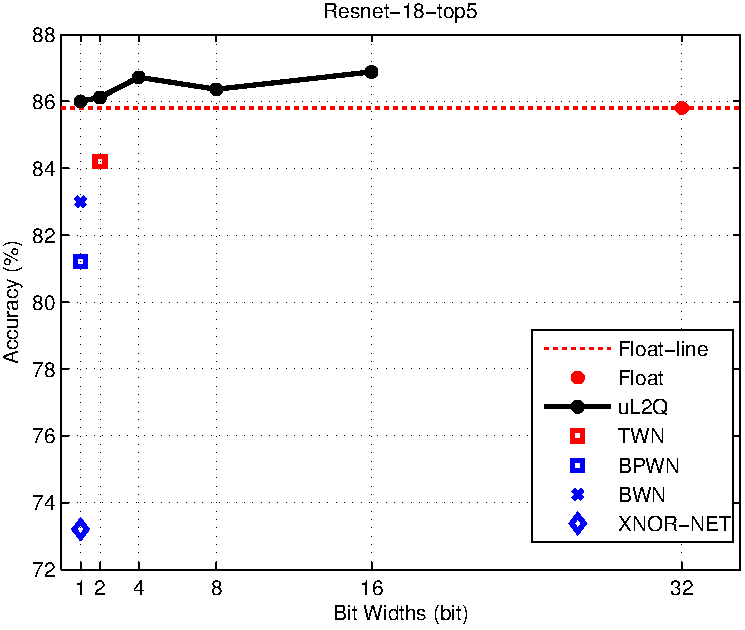
\includegraphics[width=0.31\textwidth]{fig/Resnet-18-top5_accuracy_bits.pdf}
\label{fig:resnet185acc}
}

\caption{The output accuracy of the model under different weight bit widths. The x-axis is the bit width of the model weights, and the y-axis is the output accuracy of the model. Float is the output of a full-precision weight model with 32-bit floating-point numbers, and Float-line is a horizontal line equal to the Float accuracy used for comparison.}
\label{fig:accuracy_at_bits}
\end{figure*}

\textbf{Result Analysis.} All of our comparison results are shown in Table 5. $\mu$L2Q-x and Hardware-x represent the results at x-bit width. \figref{fig:accuracy_at_bits} shows the outputs of the models at different bit widths. For objective comparison, we directly quoted the experimental results in the literature.

\textcolor{blue}{$\mu$L2Q vs Binary.} On the chosen datasets and network models, results of $\mu$L2Q at 1 bit perform better than the ones of binary methods. 
Network weights generally is not a data with standard normal distribution, but with some mean shift and standard deviation scaling. 
$\mu$L2Q is invariant about the mean shift, and is stable about the standard deviation scaling. But the binary method is unstable about these transformations, and this lead to the accuracy degradation of binary methods.

\textcolor{blue}{$\mu$L2Q vs Ternary.} At the 2 bit width, $\mu$L2Q perform better than the ternary methods, even exceed the results of float weights on some models (exceed the Float-line in \figref{fig:accuracy_at_bits}). There are two main reasons for the accuracy degradation of ternary methods. One, like the binary methods' defect, is the instability about the transformation of mean shift and the standard deviation scaling. The second reason is the waste of bit width resources. The value of ternary weights only hold three values, and its storage bit width is at least 2 bits. Meanwhile, 2 bit widths can represent up to 4 values. The expression of 4 values is much larger than 3 values, and its storage requirements are the same as the ternary. $\mu$L2Q uses four values at the 2 bit width, so its model accuracy are better than the results of the ternary methods.

\textcolor{blue}{$\mu$L2Q vs Fixed-point.} The representative method of fixed-point quantization is Hardware \citep{gysel2016hardware}. For fair comparison, we only reference the results with quantized convolution weigths in Hardware, that is, the full connection weigths are full precision. It is worth noting that Hardware had no result at 1 bit width, and its lowest bit width is 2.
Since the Mnist data set is small, Hardware and $\mu$L2Q perform similarly on Lenet5. 
On cifarnet, when the bit width is enough, the results of Hardware and $\mu$L2Q are very similar, and the accuracy degradation of both is small.
However, at low bit widths ($<4$bit), Hardware's results are poor (only 19.10\% at 2bit and 75.90\% at 4bit), and it is consistent with our prior analysis (\secref{sec:fixed-point}), that is, fixed-point quantization is poor at low bit widths. In contrast, when $\mu$L2Q at low bit widths, the results are stable. Even the result of 1bit has exceeded the result of hardware in 4bit ($\mu$L2Q-1:79.28\% $>$ Hardware-4:75.90\%).

\textcolor{blue}{$\mu$L2Q vs bitwidths} Analysis of $\mu$L2Q's results at different bit widths.
On the small network models, such as Lenet5 and Cifarnet, the accuracy of $\mu$L2Q is increasing by bit width, which is reasonable. Since the small models have less parameters, it have less redundancy,  and is easy to under-fitting. More bit widths can have more complex expressions to prevent under-fitting, so the accuracy is increasing with bit-width.
On large models, such as VGG7-64, and Resnet18, the accuracy of $\mu$L2Q is not consistent with the increase of bit width, but occur some fluctuations. $\mu$L2Q-4 outputs the highest accuracy on VGG7-64,  higher than the full precision results. $\mu$L2Q-1 has the best results on TOP1 of ResNet-18. Meanwhile, $\mu$L2Q-16 has the best results on TOP5 of ResNet-18. Large models have too many parameters, they are highly redundant and easy to over-fitting. The weights with low bit widths can reduce model complexity and prevent over-fitting,  and improve the generalization ability (test accuracy) of the model. However, too low bit widths of weights can also lead to under-fitting. Therefore, the best results of the model will only appear on the appropriate bit width.
Another interesting phenomenon is that on ResNet-18, the output accuracy of TOP1 is decreasing, while the output accuracy of TOP5 is increasing. This denotes that the redundancy of the model depends not only on the parameter number of model and the size of the data set, but also on the output of model. When the previous two conditions are given, the more complex of model's output is, the less model's redundancy is, and it is not easy to over-fitting, but easy to under-fitting. When the output is simple, it is easy to over-fitting.

%总结一下
\textcolor{blue}{$\mu$L2Q vs Float.}
$\mu$L2Q perform well on different models. Its results even are better than the ones of full precision model except Cifarnet, and it is reasonable and interpretable. These models have a certain degree of over-fitting, and low precision (bit width) of weights can reduce the complexity of the model, prevent over-fitting, and improve the generalization ability (test accuracy) of the model. Cifarnet is a special case. The parameters of the Cifarnet model are small (the parameter quantity is only 65.88\% of Lenet5), which is easy to under-fitting and needs to increase the complexity of the model to improve the performance of it. However, $\mu$L2Q is used to reduce the precision of weights and does not solve the problem of under-fitting, so it is slightly lower than the full-precision result on Cifarnet. 

%The final trained DNN performance in terms of classification accuracy is shown in Table~\ref{tab:accuracy_comp}.
%在两个模型上比全精度高
%$\mu$L2Q exceeds the output of the full precision model on both the Lenet5 and VGG7-like models. This is mainly because the two models have much parameters and great redundancy considering the data set. Therefore, quantization can remove redundancy and prevent over-fitting, which improves a certain precision.
%在Cifarnet上
%Cifarnet has few parameters, even fewer parameters than Lenet5, and its redundancy is small. The general quantization method has a great influence on the output of this model. For example, the hardware-2 (2bit) output accuracy is only 19.10\%. Meanwhile, the accuracy of $\mu$L2Q-2 (2bit) is as high as 80.26\%. Therefore, $\mu$L2Q has great advantages in low bit width quantization, and $\mu$L2Q is also ideal in high bit width.

% Please add the following required packages to your document preamble:
% \usepackage{multirow}
\begin{table}[]
\center
\caption{Accuracy(\%) comparison.}
%C is the convolutional bit width, F is the full-connection bit width, LF is the last full-connection layer bit width, and G is the gradient bit width.}
\label{tab:accuracy_comp}
\begin{tabular}{l|c|c|c|c}
\hline
Datasets    & Mnist  &\multicolumn{2}{c|}{Cifar10}   & ImageNet \\ \hline \hline
Model       & Lenet5 & Cifarnet & VGG7-like & ResNet-18(Top1/5)\\ \hline
Float       & 99.10  & 81.82    & 89.24  &65.44/85.80 \\\hline
ReBNet(M=3)\citep{ghasemzadeh2018rebnet} & -  &  -        & 86.98  &- \\
BitwiseNN\citep{BitwiseNN} &	98.67 &		- &-\\
BPWNs\citep{TWNs}  & -  &  -        & -  &57.50/81.20 \\
BWN\citep{rastegari2016xnor}  & -  &  -        & -  &60.80/83.00 \\
XNOR-NET\citep{rastegari2016xnor}  & -  &  -        & -  &51.20/73.20 \\
BC\citep{Binaryconnect}		&-&-&	88.44 &-\\\hline
TNN\citep{alemdar2017ternary}         & 98.33  &  -        & 87.89  &- \\
TrueNorth\citep{TrueNorth1} &	82.70 &		& 83.41 &- \\
TWNs\citep{TWNs}   & -  &  -        & -  &61.80/84.20 \\
STC\citep{jin2018sparse}&-&-&88.58&-\\
TC\citep{Ternaryconnect}		&-&-&	89.07&-\\\hline
Hardware-2\citep{gysel2016hardware} &	98.90 &	19.10 &-&-\\
Hardware-4\citep{gysel2016hardware} &	99.10 &	75.90 &-&-\\
Hardware-8\citep{gysel2016hardware} &	99.10 &	81.40 &-&-\\
Hardware-16\citep{gysel2016hardware} &	99.10 &	81.70 &-&-\\\hline
\textbf{$\mu$L2Q-1}       & 99.06  & 79.28    & 89.02  &66.24/86.00 \\
\textbf{$\mu$L2Q-2}       & 99.12  & 80.26    & 89.50 &65.60/86.12\\
\textbf{$\mu$L2Q-4}       & 99.12  & 81.32    & 89.80 &65.92/86.72 \\
\textbf{$\mu$L2Q-8}       & 99.16  & 81.66    & 89.70 &65.52/86.36 \\
\textbf{$\mu$L2Q-16}      & 99.14  &  81.64   & 89.42  &65.40/86.88 \\
\hline
\end{tabular}
\end{table}

%\textcolor{red}{Please add the analysis of the results in the table here. Only finish this part after your results in the table are good enough!!!}
